\documentclass[11pt]{article}
\usepackage{amsmath,amssymb,epsfig,graphics,hyperref,amsthm,mathtools,
  graphicx}
\DeclarePairedDelimiter\ceil{\lceil}{\rceil}
\DeclarePairedDelimiter\floor{\lfloor}{\rfloor}

\hypersetup{colorlinks=true}

\setlength{\textwidth}{7in}
\setlength{\topmargin}{-0.575in}
\setlength{\textheight}{9.25in}
\setlength{\oddsidemargin}{-.25in}
\setlength{\evensidemargin}{-.25in}

\reversemarginpar
\setlength{\marginparsep}{-15mm}

\newcommand{\rmv}[1]{}
\newcommand{\bemph}[1]{{\bfseries\itshape#1}}
\newcommand{\N}{\mathbb{N}}
\newcommand{\Z}{\mathbb{Z}}
\newcommand{\imply}{\to}
\newcommand{\bic}{\leftrightarrow}

% Some user defined strings for the homework assignment
%
\def\CourseCode{CS545 - Design and Analysis of Algorithms}
\def\DateHandedOut{Spring, 2015}
\def\Professor{John Kececioglu}
\def\Author{Shuo Yang}

\begin{document}

\noindent

\CourseCode \hfill \DateHandedOut

\begin{center}
Lecture Notes\\
Taught by: Professor \Professor\\
\Author\\
\end{center}

% A horizontal split line
\hrule\smallskip

\section{Divide and Conquer}
\subsection{Idea}
A Divide and Conquer algorithm consists of three phases:
\begin{enumerate}
\item Divide phase\\
Split the original problem into smaller instances of same problem
(usually $\Theta(1)$ subproblems) of size $\leq \alpha n$ for $\alpha
< 1$.
\item Conquer phase\\
Solve the subproblem recursively.
\item Combining phase\\
Combine solutions of subproblems to attain the solution to the
original problem.
\end{enumerate}

The key to applying this technique is to discover how a solution to
the input problem can be composed from (or how to decomposed into)
solution of subproblems of the same form. Problem decomposition
involves studying the structure of the solution. 

\subsection{Example}
\underline{\textbf{Largest Empty Rectangle}}\\

\underline{Input}: 2-D boolean array $A[1:m, 1:n]$ of 0s
and 1s.\\

\underline{Output}: Find a subarray $A[i:k, j:l]$ with only 0s of
largest area.\\

\underline{Exhaustive search(first attempt):} exhaustively search for
all possible rectangles that contains only 0s and find out the
largest. This takes $\Theta(n^3m^3)$ time to do, very inefficient.\\

\underline{\textbf{A divide and conquer approach:}}

Cut $A$ vertically into half at the middle column. Then the optimal
solution falls into three cases:
\begin{itemize}
\item Case-1: strictly in the left half;
\item Case-2: strictly in the right half;
\item Case-3: spans the middle.
\end{itemize}

We can recursively solve case-1 and case-2. For case-3, the largest
empty rectangle breaks into two pieces:
\begin{itemize}
\item Piece-a: left rectangle ends at mid-column and is optimal
  conditioned on starting and ending at its first and last rows. 
\item Piece-b: right rectangle starts at mid-column and is optimal
  conditioned on starting and ending at its first and last rows. 
\end{itemize}

For a given choice of row $i$ and $k$, we can find the optimal left
piece-a (starting at $i$, ending at $k$) by taking a min of the
column-left-run-length of 0s on rows $i \cdots
k$ ending at the mid-column. Similar for the optimal right piece-b. 

So we precompute:\\
$L[i,j] :=$ length of the longest run of 0s in row $i$ that ends at
$(i,j)$.\\
$R[i,j] :=$ length of the longest run of 0s in row $i$ that starts at
$(i,j)$.\\

The following pseudo code computes $L$.\\\\
\textbf{Function} $PrecomputeLeftRuns(A[1:m, 1:n])$\\
\-\hspace{2em} \textbf{for} $i := 1$ to $m$\\
\-\hspace{4em} $L[i, 0] := 0$\\
\-\hspace{4em} \textbf{for} $j := 1$ to $n$\\
\-\hspace{6em} \textbf{if} $A[i,j] == 0$\\
\-\hspace{8em} $L[i,j] := 1 + L[i, j-1]$\\
\-\hspace{6em} \textbf{else}\\
\-\hspace{8em} $L[i,j] := 0$\\

The following pseudo code computes $R$.\\\\
\textbf{Function} $PrecomputeRightRuns(A[1:m, 1:n])$\\
\-\hspace{2em} \textbf{for} $i := 1$ to $m$\\
\-\hspace{4em} \textbf{if} $A[i,n] == 0$\\
\-\hspace{6em} $R[i,n] = 1$\\
\-\hspace{4em} \textbf{else}\\
\-\hspace{6em} $R[i,n] = 0$\\
\-\hspace{4em} \textbf{for} $j := n-1$ to $1$\\
\-\hspace{6em} \textbf{if} $A[i,j] == 0$\\
\-\hspace{8em} $R[i,j] := 1 + R[i, j+1]$\\
\-\hspace{6em} \textbf{else}\\
\-\hspace{8em} $R[i,j] := 0$\\

The following pseudo code computes case-3.\\\\
\textbf{Function} $SpanningRect(A,m,lo,hi,L,R)$\\
\-\hspace{2em} $mid := \floor{\frac{hi+lo}{2}}$\\
\-\hspace{2em} $S := 0$ // holds the area of the largest empty
rectangle spanning the mid column.\\
\-\hspace{2em} \textbf{for} $i := 1$ to $m$ // row start\\
\-\hspace{4em} $minL = \infty$\\
\-\hspace{4em} $minR = \infty$\\
\-\hspace{4em} \textbf{for} $k := i$ to $m$ // row end\\
\-\hspace{6em} $minL = min(minL, L[k,mid])$\\
\-\hspace{6em} $minR = min(minR, R[k,mid])$\\
\-\hspace{6em} $S = max(S, (k-i+1) \times (minR+minL))$\\
\-\hspace{2em} \textbf{return} $S$\\

The pseudo code for divide and conquer is:\\

\textbf{Function} $LargestEmptyRect(A,m,lo,hi,L,R)$\\
\-\hspace{2em} \textbf{if} $lo < hi$ \\
\-\hspace{4em} $S := 0$\\
\-\hspace{4em} $mid := \floor{\frac{hi+lo}{2}}$\\
\-\hspace{4em} $S := max(S, LargestEmptyRect(A,m,lo,mid,L,R))$\\
\-\hspace{4em} $S := max(S, LargestEmptyRect(A,m,mid+1,hi,L,R))$\\
\-\hspace{4em} $S := max(S, SpanningRect(A,m,lo,hi,L,R))$\\
\-\hspace{4em} \textbf{return} $S$\\
\-\hspace{2em} \textbf{else} // lo == hi\\
\-\hspace{4em} \textbf{return} $LR[lo]$ // the length of longest run
of 0s in that column $A[1:m, lo]$\\

The following pseudo code computes the length of longest run of 0s for
each column, the result is in the table $LR[1:n]$.\\\\
\textbf{Function} $PrecomputeLongestRuns(A[1:m, 1:n])$\\
\-\hspace{2em} \textbf{for} $col := 1$ to $n$\\
\-\hspace{4em} \textbf{if} $A[m,col] == 0$\\
\-\hspace{6em} $prev\_run := 1$\\
\-\hspace{4em} \textbf{else}\\
\-\hspace{6em} $prev\_run := 0$\\
\-\hspace{4em} max\_run := prev\_run\\
\-\hspace{4em} \textbf{for} $i := m-1$ to $1$\\
\-\hspace{6em} \textbf{if} $A[i,col] == 0$\\
\-\hspace{8em} $curr\_run := 1 + prev\_run$\\
\-\hspace{6em} \textbf{else}\\
\-\hspace{8em} $curr\_run := 0$\\
\-\hspace{6em} $max\_run = max(max\_run, curr\_run)$\\
\-\hspace{6em} $prev\_run = curr\_run$\\
\-\hspace{4em} $LR[col] := max\_run$\\

Putting together, the final pseudo code is:\\

\textbf{Function} $FindLargestEmptyRect(A,m,lo,hi,L,R)$\\
\-\hspace{3em} $L := PrecomputeLeftRuns(A)$\\
\-\hspace{3em} $R := PrecomputeRightRuns(A)$\\
\-\hspace{3em} $LR := PrecomputeLongestRuns(A)$\\
\-\hspace{3em} \textbf{return} $LargestEmptyRect(A,m,1,n,L,R,LR)$\\

\underline{Run time analysis:}\\
Subroutine $PrecomputeLeftRuns$, $PrecomputeRightRuns$ and
$PrecomputeLongestRuns$ all take $\Theta(mn)$ time. Subroutine
$SpanningRect$ takes $\Theta(m^2)$ time, so the recurrence equation
for the routine $LargestEmptyRect$ is:

\begin{equation}
\begin{split}
  T(m,n) &= T(m,\frac{n}{2}) + T(m,\frac{n}{2}) + \Theta(m^2)\\
  &= 2T(m,\frac{n}{2}) + \Theta(m^2)\\
  &= \Theta(nm^2)
\end{split}
\end{equation}

The intuition behind this result is that since $m$ does not change for
$n$, so we can treat $m$ as constant for $n$. This yields a simple
recurrence equation:

\begin{equation}
\begin{split}
  T(n) &= 2T(\frac{n}{2}) + \Theta(1)\\
  &= \Theta(n)
\end{split}
\end{equation}

Since the algorithm always spends $\Theta(m^2)$ for each subproblem,
therefore the total run time is $\Theta(n)\Theta(m^2) = \Theta(nm^2)$.

\underline{\textbf{To summarize:}}\\

All possible rectangles in $A[1:m,1:n]$ is $\Theta(m^2n^2)$. Our
divide-and-conquer algorithm guarantees not to look at all possible
rectangles. The key is case-3, where we first find the best left
rectangle, and then the best right rectangle, then just glue them
together, in doing so we can avoid searching for all possible
rectangles. \\

Another insight is that every rectangle spans some column, so for
every column $j$, we just ask: what is the longest rectangle spanning
$j$, so the total run time is $\Theta(nm^2)$.\\

\underline{\textbf{Comparison of different algorithms}}\\

\begin{center}
    \begin{tabular}{ | l | l |}
    \hline
    Algorithm & Run time \\ \hline
    Exhaustive search & $\Theta(m^3n^3)$ (can be reduced to
    $\Theta(m^2n^2)$) \\ \hline
    Divide and conquer & $\Theta(mn \times min(m,n))$ (depends on
    dividing horizontally or vertically) \\ \hline
    Dynamic programming & $\Theta(mn \times min(m,n))$ \\ \hline
    Amortized & $\Theta(mn)$ (this is optimal algorithm, have to look
    at every entry?) \\ \hline
    \end{tabular}
\end{center}

\section{Finding $k_{th}$ smallest}
\subsection{Finding minimum and maximum simultaneously}

\underline{algorithm using $2n-2$ comparisons}\\

\textbf{Function} $MinMax(A[1:n])$\\
\-\hspace{3em} $min := A[1]$\\
\-\hspace{3em} $max := A[1]$\\
\-\hspace{3em} \textbf{for} $i := 2$ to $n$\\
\-\hspace{5em} \textbf{if} $A[i] < min$\\
\-\hspace{7em} $min := A[i]$\\
\-\hspace{5em} \textbf{if} $A[i] > max$\\
\-\hspace{7em} $max := A[i]$\\
\-\hspace{3em} \textbf{return} $(min,max)$\\

\underline{algorithm using $3\floor{n/2}$ comparisons}\\

\textbf{Function} $MinMax(A[1:n])$\\
\-\hspace{3em} \textbf{if} $n$ is odd\\
\-\hspace{5em} $min := A[1]$\\
\-\hspace{5em} $max := A[1]$\\
\-\hspace{3em} \textbf{else}\\ 
\-\hspace{5em} \textbf{if} $A[1] > A[2]$\\
\-\hspace{7em} $min := A[2]$\\
\-\hspace{7em} $max := A[1]$\\
\-\hspace{5em} \textbf{else}\\ 
\-\hspace{7em} $min := A[1]$\\
\-\hspace{7em} $max := A[2]$\\
\-\hspace{3em} \textbf{while} $i \leq n-1$\\
\-\hspace{5em} \textbf{if} $A[i] < A[i+1]$\\
\-\hspace{7em} \textbf{if} $A[i] < min$\\
\-\hspace{9em} $min := A[i]$\\
\-\hspace{7em} \textbf{if} $A[i+1] > max$\\
\-\hspace{9em} $max := A[i+1]$\\
\-\hspace{5em} \textbf{else}\\
\-\hspace{7em} \textbf{if} $A[i+1] < min$\\
\-\hspace{9em} $min := A[i+1]$\\
\-\hspace{7em} \textbf{if} $A[i] > max$\\
\-\hspace{9em} $max := A[i]$\\
\-\hspace{5em} $i := i+2$\\
\-\hspace{3em} \textbf{return} $(min, max)$\\

\subsection{Finding $k_{th}$ smallest in $\Theta(n)$ worst-case time}

The algorithm works as follows:\\

\textbf{Function} $k_{th}Smallest(A[1:n], k)$\\
\-\hspace{3em} $med := FindMedian(A[1:n])$\\
\-\hspace{3em} $Partition(A[1:n], med)$\\
\-\hspace{3em} \textbf{if} $k == \ceil{\frac{n}{2}}$\\
\-\hspace{5em} \textbf{return} $med$\\
\-\hspace{3em} \textbf{else if} $k < \ceil{\frac{n}{2}}$\\
\-\hspace{5em} \textbf{return}
$k_{th}Smallest(A[1:\ceil{\frac{n}{2}}-1], k)$\\
\-\hspace{3em} \textbf{else}\\
\-\hspace{5em} \textbf{return}
$k_{th}Smallest(A[\ceil{\frac{n}{2}}+1:n], k-\ceil{\frac{n}{2}})$\\


\section{Greedy Algorithm}
\subsection{Activity selection problem}

\emph{input:} a collection of $n$ activities, that are competing for a
single resource, and must be scheduled. Activity $i$ has a start time
$s_i$ and finish time $f_i$, where $s_i \leq f_i$, and it wishes to
use the resource during $[s_i, f_i)$. Activities $i$ and $j$ are
compatible if their intervals $[s_i, f_i)$ and $[s_j, f_j)$ do not
overlap. 

The activity selection problem is to choose a subset of mutually
compatible activities of maximum cardinality. \\

\underline{Greedy algorithm strategy}\\

Let us order the activities by increasing finish time: $f_1 \leq f_2
\leq \cdots \leq f_n$. Consider the activities in this order (earliest
finish time first), and add on to our subset if it is compatible with
our subset. The following algorithm implements this idea where $S$ and
$F$ are sets of start time and finish time sorted by increasing finish
time, $n$ is the number of activities.\\

\textbf{Function} $GreedyActivitySelection(S, F, n)$\\
\-\hspace{3em} $A := \{1\}$ // earliest finished activity\\
\-\hspace{3em} $j := 1$ // indicates the latest finish time in $A$\\
\-\hspace{3em} \textbf{for} $i := 2$ to $n$ \\
\-\hspace{5em} \textbf{if} $S[i] \geq F[j]$ \\
\-\hspace{7em} $A := A \cup \{i\}$ \\
\-\hspace{7em} $j := i$ \\
\-\hspace{3em} \textbf{return} $A$ \\

\underline{Correctness}\\\\
\textbf{Lemma:} Suppose $A$ is a subset of an optimal solution. Let
$a$ be an activity that finishes earliest among all activities that
are compatible with $A$ and that finish after the activities in
$A$. Then $A \cup {a}$ is also a subset of an optimal solution.

\begin{proof}
  Since $A$ is a subset of an optimal solution, let $A^*$ be an
  optimal solution with $A \subseteq A^*$. Let $b$ be the activity in
  $A^* - A$  that also finishes earliest among those finish after the
  activities in $A$. We have two cases:
\begin{itemize}
\item case-1: $b = a$, then $A \cup \{a\} \subseteq A^*$, the lemma
  holds. 
\item case-2: $b \neq a$, then $b$ must finish after $a$. We can
  substitute $a$ for $b$ in $A^*$ and still yields an optimal
  solution. Thus $(A^* - \{b\}) \cup \{a\}$ is a mutually compatible
  set with the same cardinality as $A^*$, so it is also an optimal
  solution, and moreover, it contains $A \cup \{a\}$.
  
  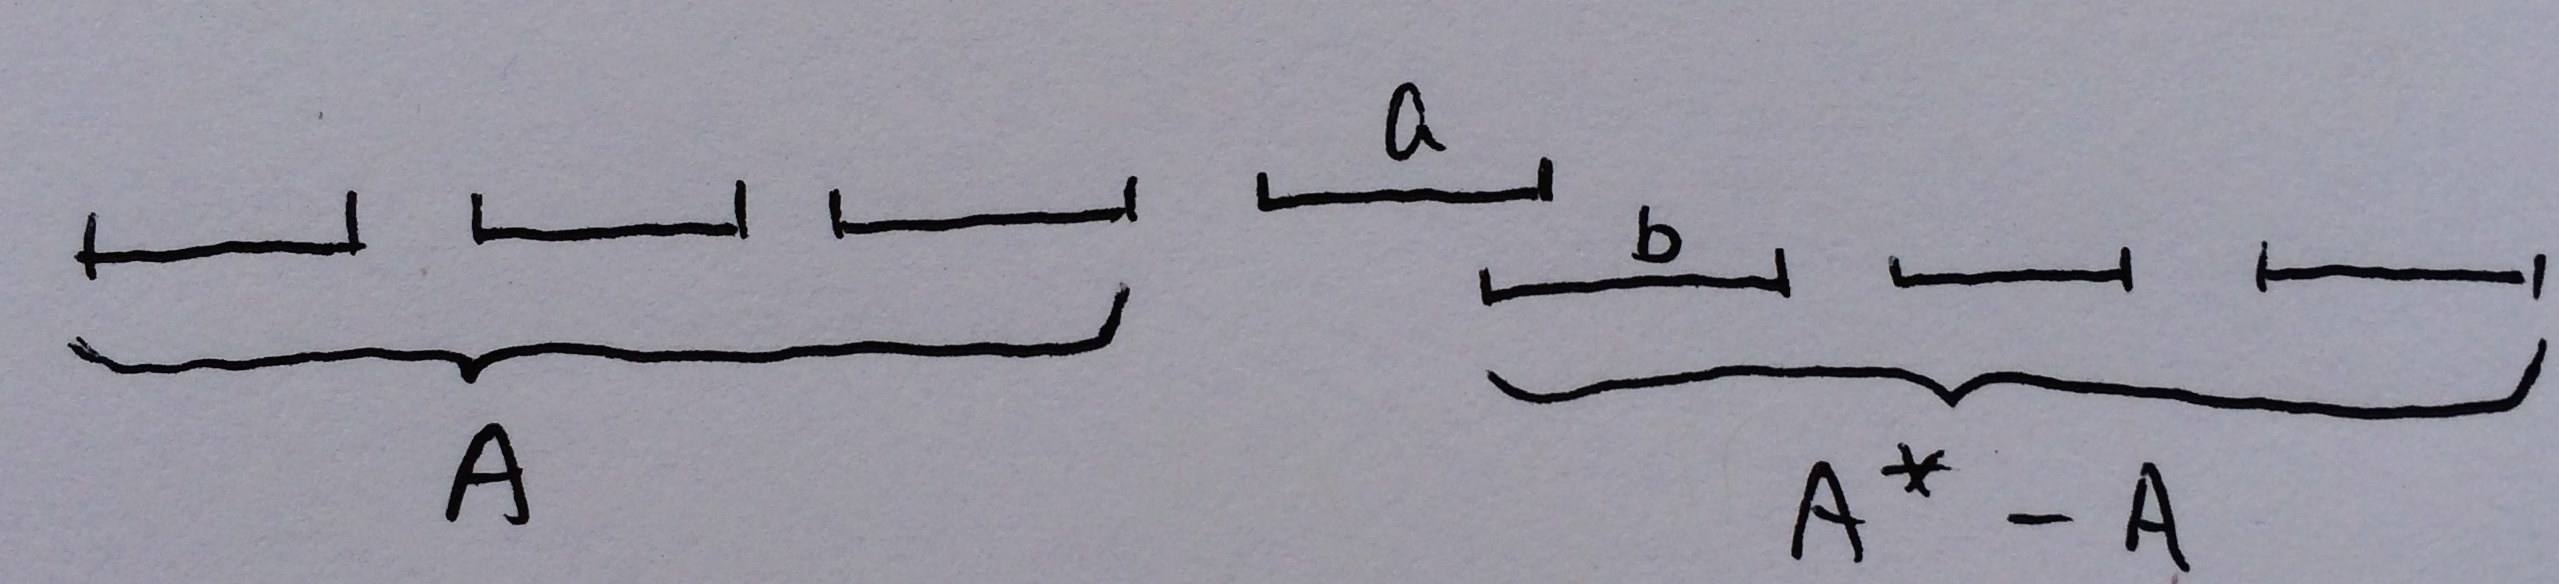
\includegraphics[width=7cm,height=2cm]{./imgs/activity-selection.png}
  
\end{itemize}
\end{proof}

\textbf{Theorem:} $GreedyActivitySelection$ finds an optimal
solution. 

\begin{proof}
  Certainly, $\emptyset$ is always a subset of an optimal
  solution. Thus $\emptyset \cup \{1\}$ is a subset of an optimal
  solution by the lemma. 

  By induction on the number of iteration, when the function
  terminates, $A$ is a subset of an optimal solution. And all
  activities not in $A$ are incompatible with some activity in $A$, so
  $A$ is not properly contained by any solution. Thus $A$ is optimal. 
\end{proof}

\subsection{Proving correctness in general for greedy algorithm}

When analyzing the correctness of a greedy algorithm, first prove a
lemma of the following form:\\

\underline{\textbf{Greedy Augmentation Lemma:}}\\
Suppose $S$ is contained in an optimal solution. Let $S'$ be an
augmentation of $S$ produced by one step of the greedy algorithm. Then
$S'$ is also contained in the optimal solution.\\

We can prove the lemma by \emph{exchange-style-argument:} if the
optimal solution does not contain $S'$, then make an exchange between
the augmented element in $S'$ and an element in the optimal solution
to produce another optimal solution since it did not get worse.\\

Notice that we need to define the containment relationship for the
specific problem. It could be over set, or over string(substring,
prefix, suffix, etc).\\

Finally, the full correctness proof of a greedy algorithm will then
consist of 4 steps:
\begin{enumerate}
\item argue the initial state (usually $\emptyset$) is contained in an
  optimal solution.
\item using induction on the number of augmentations of greedy
  algorithm, use the lemma, argue that the output $S$ of the greedy
  algorithm is contained in an optimal solution.
\item show that there exists no optimal solution that can properly
  contain $S$.
\end{enumerate}

\end{document}
